\section{Cabling in rack cabinet}

\renewcommand{\CURPATH}{MaxSxT/cabling}

Take a rack cabinet, like this one:

\begin{figure}[H]
\centering
\frame{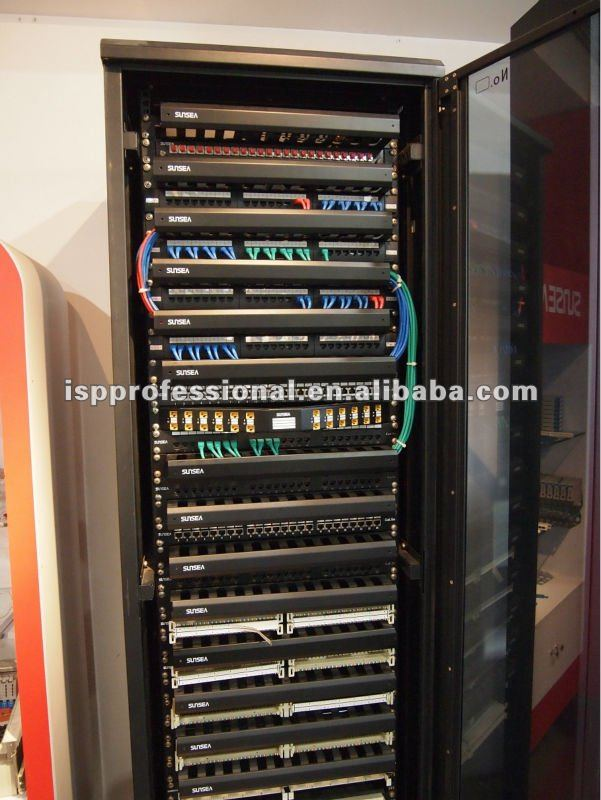
\includegraphics[scale=0.7]{\CURPATH/1.jpg}}
\end{figure}

Let's say, there are 8 1U devices, maybe servers, routers and whatnot, named as A, B, C, D, E, F, G, H.
Devices must be connected by cables: probably twisted pair or whatever network engineers using today.
Some devices must be connected by several cables (2 cables, 3 or 4):

\begin{lstlisting}
A <--- 1 cable  ---> H
A <--- 2 cables ---> E
B <--- 4 cables ---> F
C <--- 1 cable  ---> G
C <--- 1 cable  ---> D
C <--- 1 cable  ---> E
D <--- 3 cables ---> H
G <--- 1 cable  ---> H
\end{lstlisting}

The problem: how we can place these 8 devices in such an order, so that sum of all cable lengths would be as short as possible?

\lstinputlisting[style=custompy]{\CURPATH/cabling.py}

Each 1 in \verb|diff_X_X| variables and in \verb|final_sum| means a cable of length enough to connect two 1U devices placed adjacently.
So we measure cable lengths in \emph{units}.

Minimizing:

\lstinputlisting{\CURPATH/min.txt}

So we need a cable of 19 units to cut it and connect everything.

Essentially, we're asking Z3 to find such values for A, B, C, D, E, F, G, H, so that the value of the following expression would be as small as possible:

\begin{lstlisting}
diff_A_H +                                                                                                             
diff_A_E*2 +
diff_B_F*4 +
diff_C_G +
diff_C_D +
diff_C_E +
diff_D_H*3 +
diff_G_H
\end{lstlisting}

Just for fun, we can maximize solution (comment \verb|s.minimize()| and uncomment \verb|s.maximize()|):

\lstinputlisting{\CURPATH/max.txt}

Further work: it's not a problem to extend this script for several types of cables: network, power, etc, and minimize them as well.
Even more, we can assign priorities: maybe, we can live with longer network cables, but want to minimize lengths of power cables at first,
or vice versa.

